\documentclass[tikz,border=1cm]{standalone}
\usepackage{amsmath}
\usetikzlibrary{quotes,arrows.meta,decorations.pathreplacing}
\tikzset{
    line cap=round,line join=round,
    annoted cuboid/.pic={%
        \tikzset{%
            every edge quotes/.append style={auto},
            /cuboid/.cd,#1,
        }
    \draw[every edge/.append style={pic actions, densely dashed, opacity=.5},pic actions]
    (0,0,0) coordinate (o) -- 
    ++(-\cubescale*\cubex,0,0) coordinate (a) --
    ++(0,-\cubescale*\cubey,0) coordinate (b) edge coordinate[pos=1] (g)
    ++(0,0,-\cubescale*\cubez) --
    ++(\cubescale*\cubex,0,0) coordinate (c) -- cycle
    (o) -- ++(0,0,-\cubescale*\cubez) coordinate (d) -- 
    ++(0,-\cubescale*\cubey,0) coordinate (e) edge (g) -- (c) -- cycle
    (o) -- (a) -- ++(0,0,-\cubescale*\cubez) coordinate (f) edge (g) -- (d) -- cycle;

    \ifnum\br=0 \relax
    \else\path[every edge/.append style={pic actions,decoration=brace,decorate,fill=none}]
    (c) +(0,-2pt) coordinate(c1) edge node[midway,below]{\cubewt} (c1 -| b)
    (b) +(-2pt,0) coordinate(b2) edge node[midway,left]{\cubeht} (b2 |- a)
    (e) +(1.5pt,-1.5pt) coordinate(c2) edge node[midway,right,yshift=-2pt] {\cubezt} ([xshift=1.5pt,yshift=-1.5pt]c);
    \fi
},
    /cuboid/.cd,
    /cuboid/.search also={\tikz},
    width/.store in=\cubex,
    height/.store in=\cubey,
    depth/.store in=\cubez,
    widthtext/.store in =\cubewt,
    heighttext/.store in=\cubeht,
    depthtext/.store in=\cubezt,
    scale/.store in=\cubescale,
    brace/.store in=\br,
    width=10,height=10,
    depth=10,scale=.1,brace=1,
}
\begin{document}
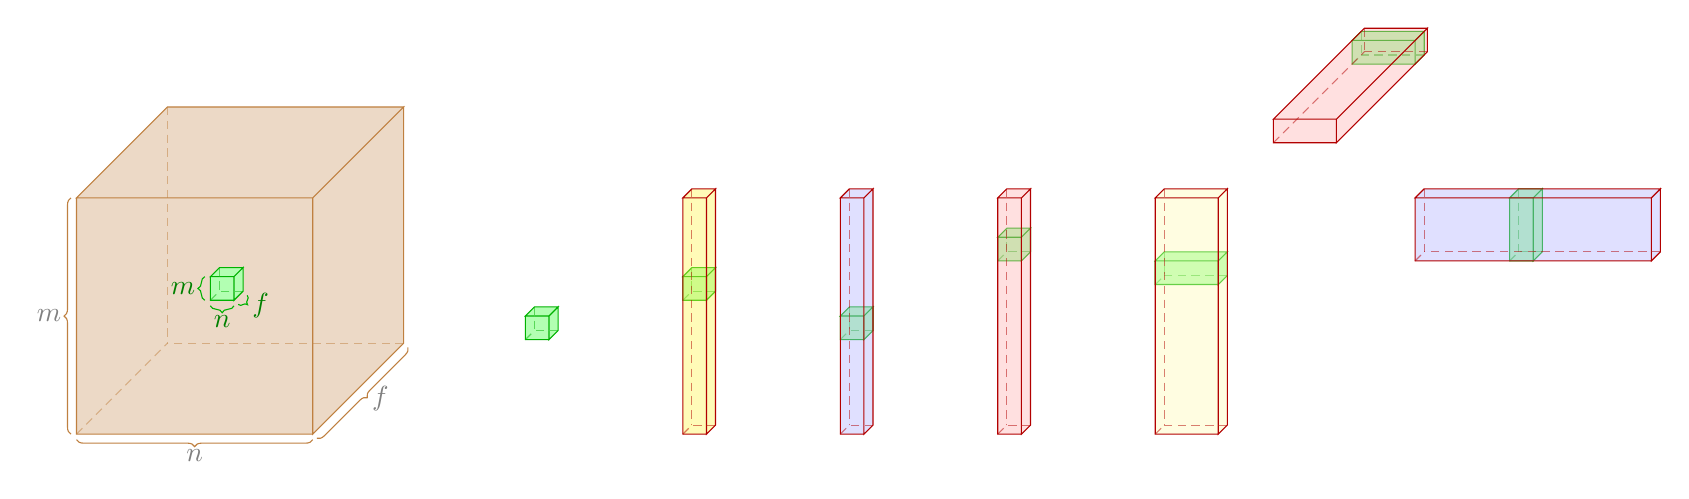
\begin{tikzpicture}
    \pic [fill=brown!30!white, text=gray, draw=brown] at (0,0)
    {annoted cuboid={width=30,height=30,depth=30,widthtext=$n$,heighttext=$m$,depthtext=$f$,brace=1}};
    \pic [fill=green!30!white, text=black!50!green, draw=black!30!green] at (-1,-1)
    {annoted cuboid={width=3,height=3,depth=3,widthtext=$n$,heighttext=$m$,depthtext=$f$,brace=1}};

    \pic [fill=green!30!white, text=black!50!green, draw=black!30!green] at (3,-1.5)
    {annoted cuboid={width=3,height=3,depth=3,widthtext=,heighttext=,depthtext=,brace=0}};

    \pic [fill=green!30!white, text=black!50!green, draw=black!30!green] at (5,-1)
    {annoted cuboid={width=3,height=3,depth=3,widthtext=,heighttext=,depthtext=,brace=0}};
    \pic [fill=white!30!yellow, fill opacity=0.4, text=black!50!green, draw=black!30!red] at (5,0)
    {annoted cuboid={width=3,height=30,depth=3, widthtext=,heighttext=,depthtext=,brace=0}};

    \pic [fill=green!30!white, text=black!50!green, draw=black!30!green] at (7,-1.5)
    {annoted cuboid={width=3,height=3,depth=3,widthtext=,heighttext=,depthtext=,brace=0}};
    \pic [fill=white!70!blue, fill opacity=0.4, text=black!50!green, draw=black!30!red] at (7,0)
    {annoted cuboid={width=3,height=30,depth=3, widthtext=,heighttext=,depthtext=,brace=0}};

    \pic [fill=green!30!white, text=black!50!green, draw=black!30!green] at (9,-0.5)
    {annoted cuboid={width=3,height=3,depth=3,widthtext=,heighttext=,depthtext=,brace=0}};
    \pic [fill=white!70!red, fill opacity=0.4, text=black!50!green, draw=black!30!red] at (9,0)
    {annoted cuboid={width=3,height=30,depth=3, widthtext=,heighttext=,depthtext=,brace=0}};

    \pic [fill=green!30!white, text=black!50!green,draw=black!30!green] at (11.5,-0.8)
    {annoted cuboid={width=8,height=3,depth=3,widthtext=,heighttext=,depthtext=,brace=0}};
    \pic [fill=white!70!yellow, fill opacity=0.4, text=black!50!green, draw=black!30!red] at (11.5,0)
    {annoted cuboid={width=8,height=30,depth=3,widthtext=,heighttext=,depthtext=,brace=0}};

    \pic [fill=green!30!white, text=black!50!green,draw=black!30!green] at (14,2)
    {annoted cuboid={width=8,height=3,depth=3,widthtext=,heighttext=,depthtext=,brace=0}};
    \pic [fill=white!70!red, fill opacity=0.4, text=black!50!green, draw=black!30!red] at (13,1)
    {annoted cuboid={width=8,height=3,depth=30,widthtext=,heighttext=,depthtext=,brace=0}};

    \pic [fill=green!30!white, text=black!50!green,draw=black!30!green] at (15.5,0)
    {annoted cuboid={width=3,height=8,depth=3, widthtext=,heighttext=,depthtext=,brace=0}};
    \pic [fill=white!70!blue, fill opacity=0.4, text=black!50!green, draw=black!30!red] at (17,0)
    {annoted cuboid={width=30,height=8,depth=3, widthtext=,heighttext=,depthtext=,brace=0}};
\end{tikzpicture}

\end{document}